\documentclass[paper=a4, fontsize=11pt]{scrartcl} % KOMA-article class

%-------------------------------------------------
%   THEMES, PACKAGES, CUSTOM COMMANDS
%-------------------------------------------------
\usepackage{blindtext}
\usepackage[english]{babel}                             % English language/hyphenation
\usepackage[protrusion=true,expansion=true]{microtype}  % Better typography
\usepackage{amsmath,amsfonts,amsthm}                    % Math packages
\usepackage[pdftex]{graphicx}                           % Enable pdflatex
\usepackage[export]{adjustbox}
\usepackage[svgnames]{xcolor}                           % Enabling colors by their 'svgnames'
\usepackage[hang, small,labelfont=bf,up,textfont=it,up]{caption} % Custom captions under/above floats
\usepackage{subcaption}
\usepackage{caption}
\usepackage{epstopdf}       % Converts .eps to .pdf
%\usepackage{subfig}         % Subfigures
\usepackage{booktabs}       % Nicer tables
\usepackage{fix-cm}         % Custom fontsizes
\usepackage{listings}
\usepackage{soul}
\usepackage{float}

\usepackage{hyperref}

\usepackage[foot=30pt,margin=1in]{geometry}

% Custom sectioning (sectsty package)
\usepackage{sectsty}
\allsectionsfont{
    \usefont{OT1}{phv}{b}{n}    % bch-b-n: CharterBT-Bold font
}
\sectionfont{
    \usefont{OT1}{phv}{b}{n}
}

% Custom colors
\definecolor{brsugrey}{rgb}{0.9, 0.9, 0.9}
\definecolor{brsublue}{rgb}{0, 0.594, 0.949}

%
\newcommand{\upperRomannumeral}[1]{\uppercase\expandafter{\romannumeral#1}}

% Creating an initial of the very first character of the content
\usepackage{lettrine}
\newcommand{\initial}[1]{%
    \lettrine[lines=3,lhang=0.3,nindent=0em]{
        \color{brsublue}
        {\textsf{#1}}}{}}

%-------------------------------------------------
%   COMMON INFO
%-------------------------------------------------
\newcommand{\hmwkTitle}{Assignment \upperRomannumeral{3} - Shape Matching}
\newcommand{\hmwkDueDate}{Thursday, 25 May 2017}
\newcommand{\hmwkClass}{Evolutionary Computation Theory and Application}
\newcommand{\hmwkClassShort}{ECTA SS17}
\newcommand{\hmwkAuthorFullName}{Minh H. Nguyen \& Pranjal Dhole}
\newcommand{\hmwkAuthorLastName}{Nguyen \& Dhole}
\newcommand{\hmwkAuthorEmail}{minh.nguyen@smail.inf.h-brs.de}
\newcommand{\hmwkAuthorInstitute}{BRS University of Applied Sciences}
\newcommand{\headerFontSize}{19}
\graphicspath{{images/}}

%-------------------------------------------------
%   HEADERS & FOOTERS
%-------------------------------------------------
\usepackage{fancyhdr}
\pagestyle{fancy}
\usepackage{lastpage}
% Header (empty)
\lhead{}
\chead{}
\rhead{}
% Footer (you may change this to your own needs)
\lfoot{\footnotesize
    \texttt{\hmwkClassShort} ~
    \textbullet ~ \hmwkAuthorLastName ~
    \textbullet ~ \hmwkTitle}
\cfoot{}
\rfoot{\footnotesize page \thepage\ of \pageref{LastPage}}  % "Page 1 of 2"
\renewcommand{\headrulewidth}{0.0pt}
\renewcommand{\footrulewidth}{0.4pt}

%-------------------------------------------------
%   TITLE & AUTHOR
%-------------------------------------------------
\usepackage{titling}

\newcommand{\HorRule}{\color{brsublue}% Creating a horizontal rule
    \rule{\linewidth}{1pt}%
    \color{black}
}

% Title
\pretitle{
    \vspace{-30pt}
    \begin{flushleft}
        \HorRule
        \fontsize{\headerFontSize}{\headerFontSize} \usefont{OT1}{phv}{b}{n} \color{gray} \selectfont
}
\title{\hmwkClass \\
       \hmwkTitle}
\posttitle{
    \par
    \end{flushleft}
    \vskip 0.5em
}

% Author
\preauthor{
    \begin{flushleft}
        \large \lineskip 0.25em
        \usefont{OT1}{phv}{b}{sl} \color{brsublue}}

\author{\hmwkAuthorFullName}

\postauthor{
        \footnotesize
        \usefont{OT1}{phv}{m}{sl} \color{Black}
        \\\hmwkAuthorInstitute
        \\\hmwkAuthorEmail
        \par
    \end{flushleft}
    \HorRule}

% Date
\date{\hmwkDueDate}

%-------------------------------------------------
%   BEGIN
%-------------------------------------------------
\begin{document}
    \maketitle
    \thispagestyle{fancy}

    \section{Hyper parameters}

    \begin{tabular}{ll}
        Population size ($\lambda$) & $15$ \\
        Number of genes ($N$)       & 32 \\
        Number of generations       & $1200$ \\
        Step size ($\sigma$)        & $0.3$ \\
        $\mu$ ($\lambda / 2$)       & $7$ \\
        weights ($w_i \propto (\mu - i + 1)$)
                                    & $\left[ \begin{matrix}
                                      0.2381 & 0.2063 & 0.1746 & 0.1429 & 0.1111 & 0.0794 & 0.0476
                                      \end{matrix} \right]$ \\
        $\mu_{eff}$ ($1 / \sum w_i^2$)
                                    & $5.845$ \\
        $c_\mu$ ($\mu_{eff} / N^2$) & $0.0057$ \\
    \end{tabular}

    \section{Solution}
    \begin{figure}[H]
        \centering
        \begin{minipage}{.5\textwidth}
            \centering
            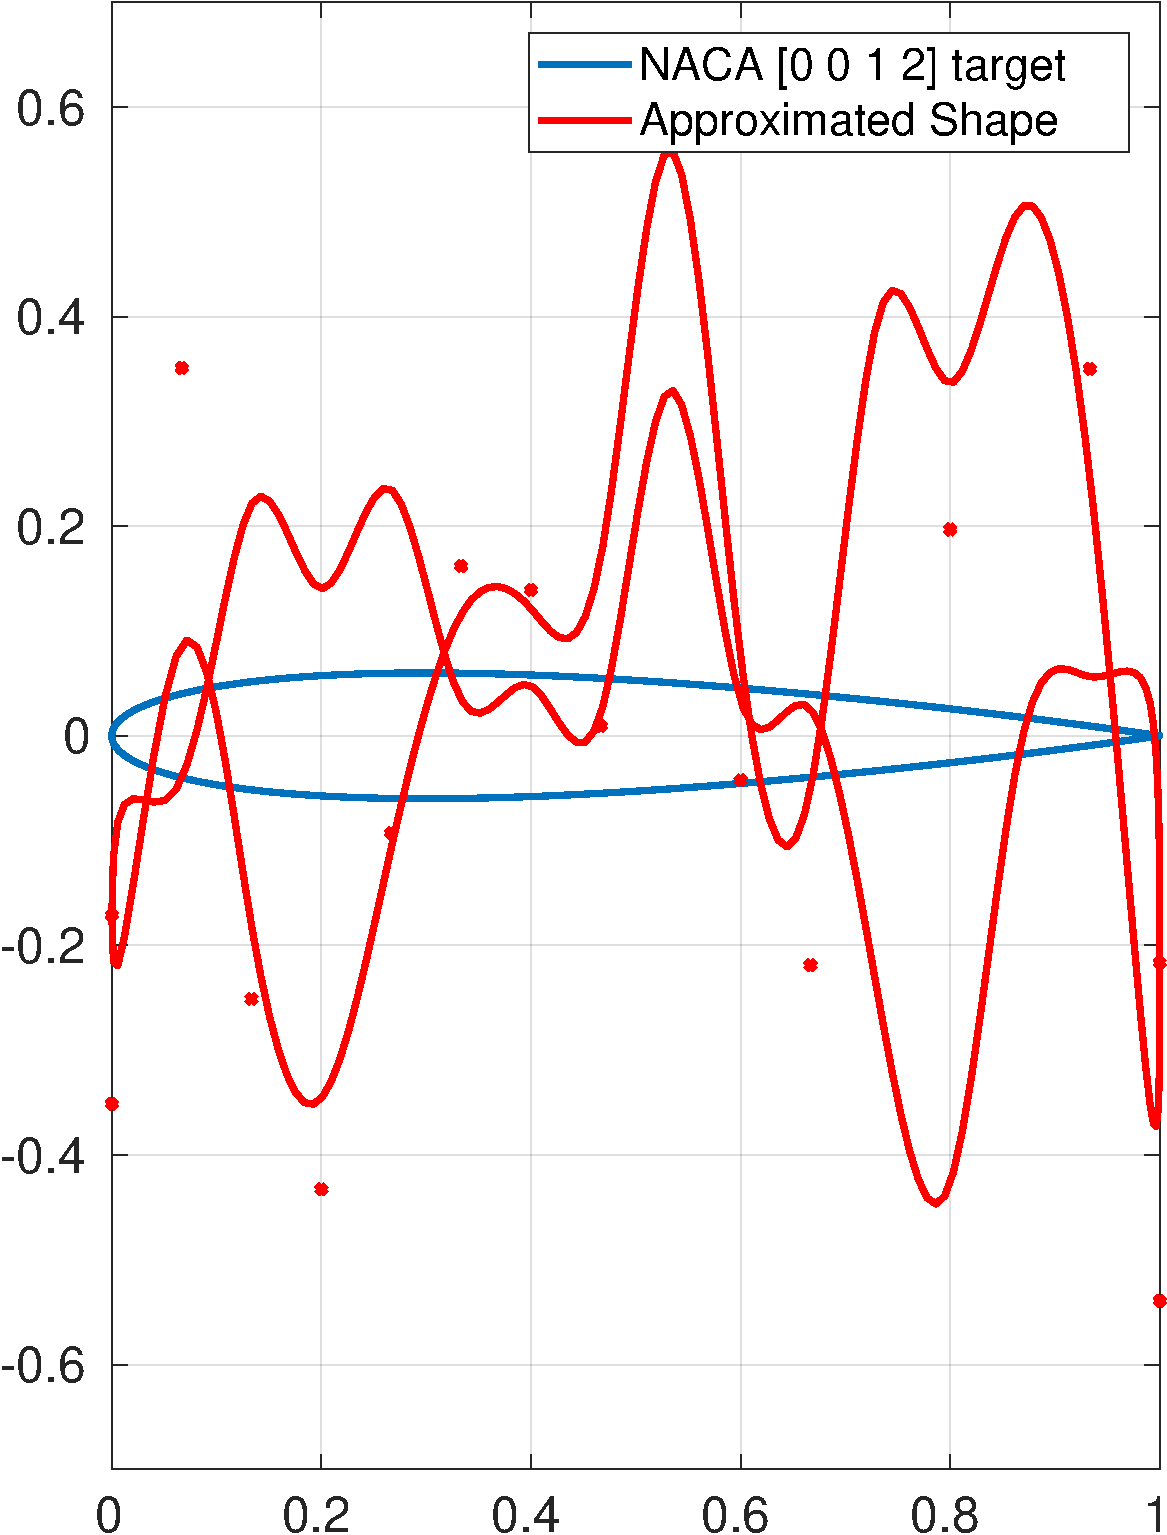
\includegraphics[width=.95\linewidth]{a3-shapematch-0012-init}
            \captionof{figure}{Initialized solution for the 0012 shape}
            \label{fig:initial0012}
        \end{minipage}%
        \begin{minipage}{.5\textwidth}
            \centering
            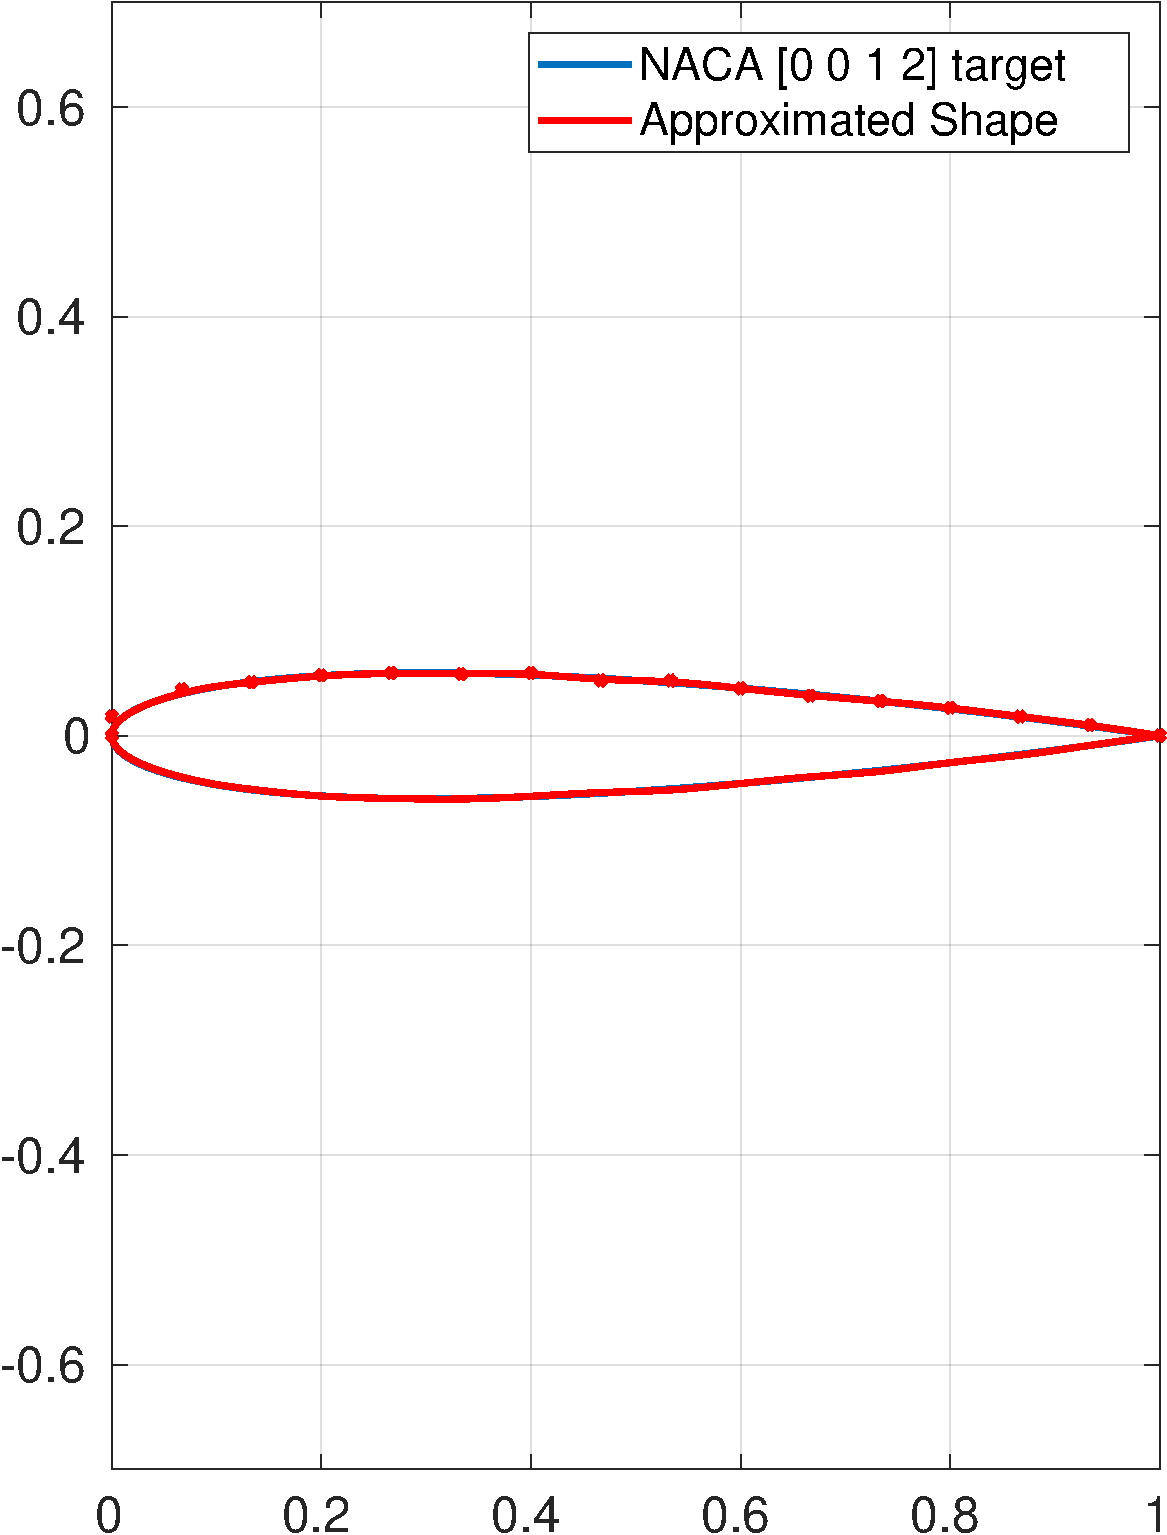
\includegraphics[width=.95\linewidth]{a3-shapematch-0012-final}
            \captionof{figure}{A final solution for the 0012 shape}
            \label{fig:solution0012}
        \end{minipage}
    \end{figure}

    \begin{figure}[H]
        \centering
        \begin{minipage}{.5\textwidth}
            \centering
            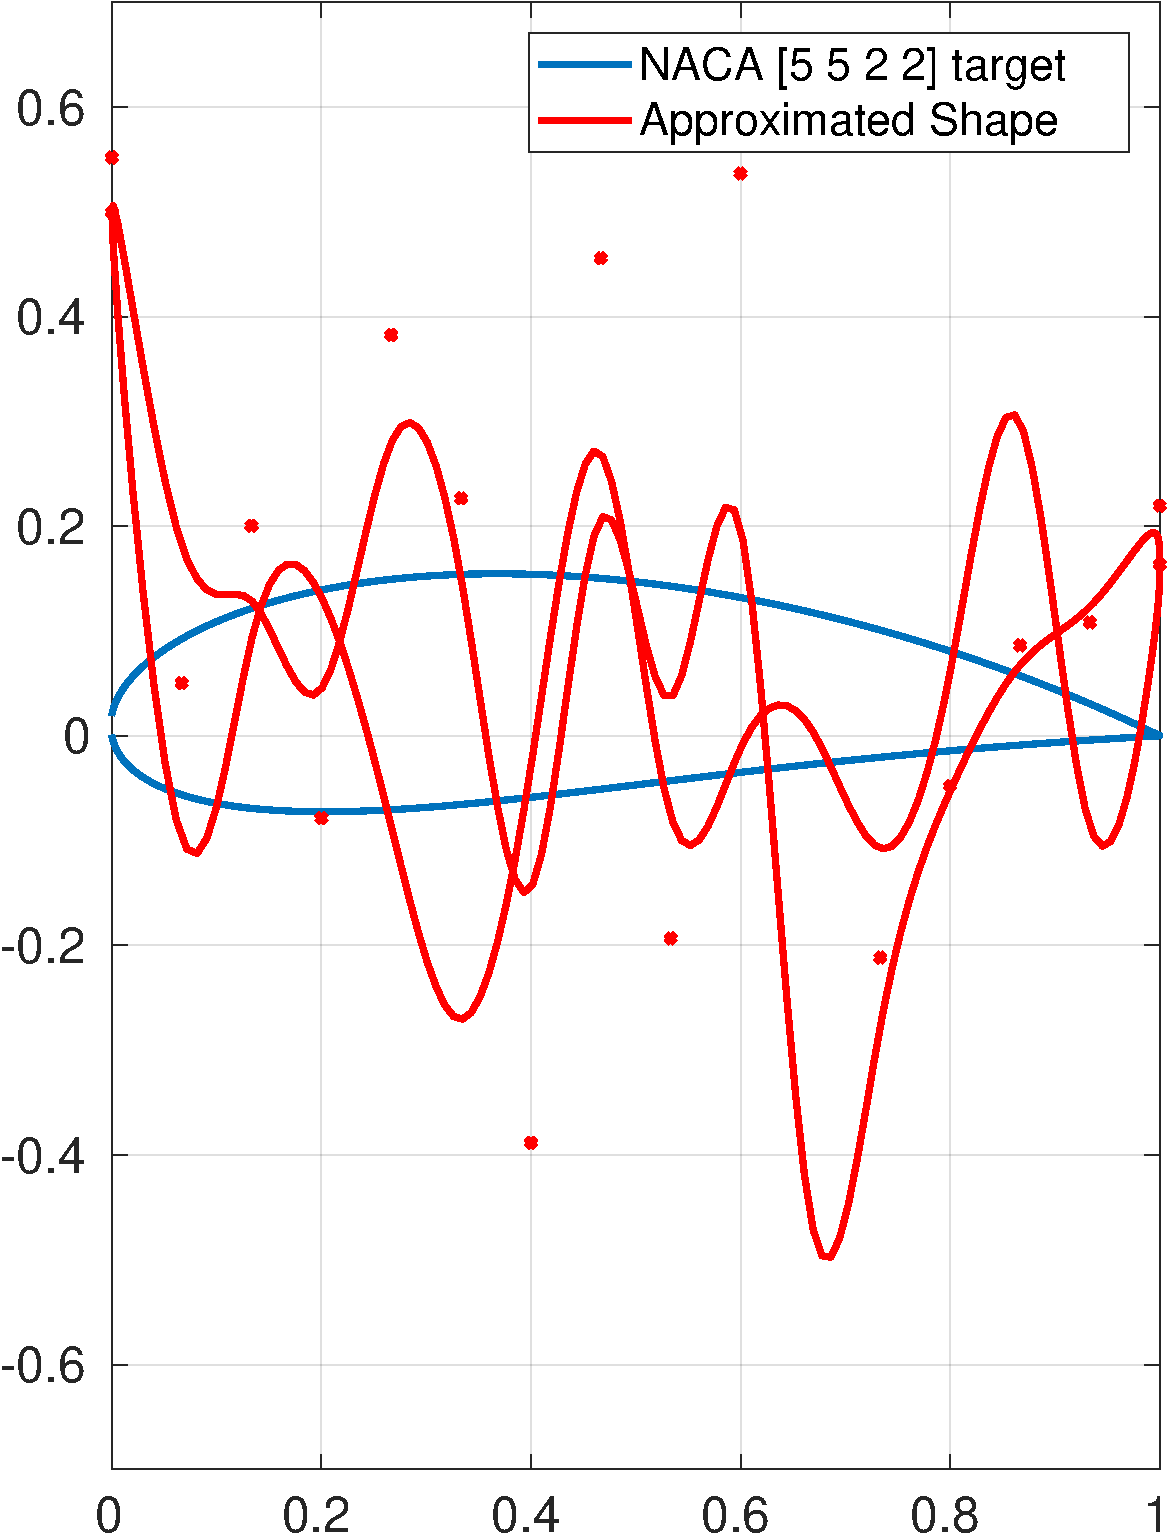
\includegraphics[width=.95\linewidth]{a3-shapematch-5522-init}
            \captionof{figure}{Initialized solution for the 5522 shape}
            \label{fig:initial5522}
        \end{minipage}%
        \begin{minipage}{.5\textwidth}
            \centering
            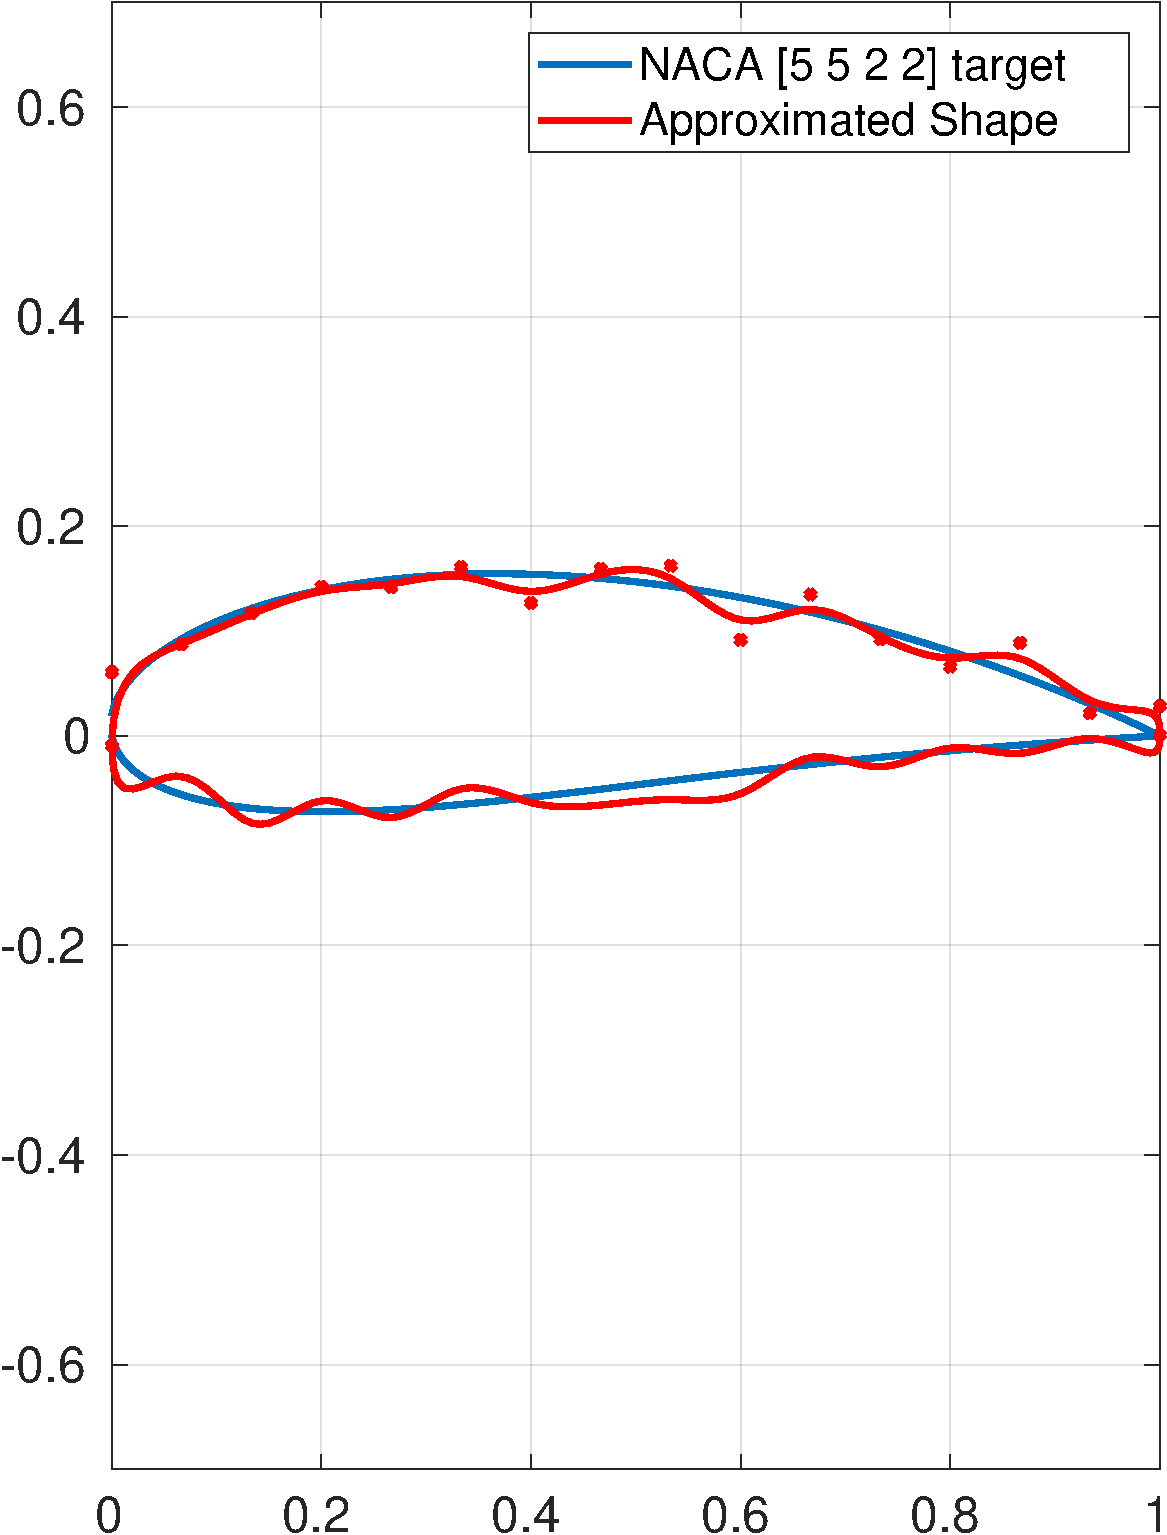
\includegraphics[width=.95\linewidth]{a3-shapematch-5522-final}
            \captionof{figure}{A final solution for the 5522 shape}
            \label{fig:solution5522}
        \end{minipage}
    \end{figure}

    \begin{figure}[H]
    \centering
    \begin{minipage}{.5\textwidth}
        \centering
        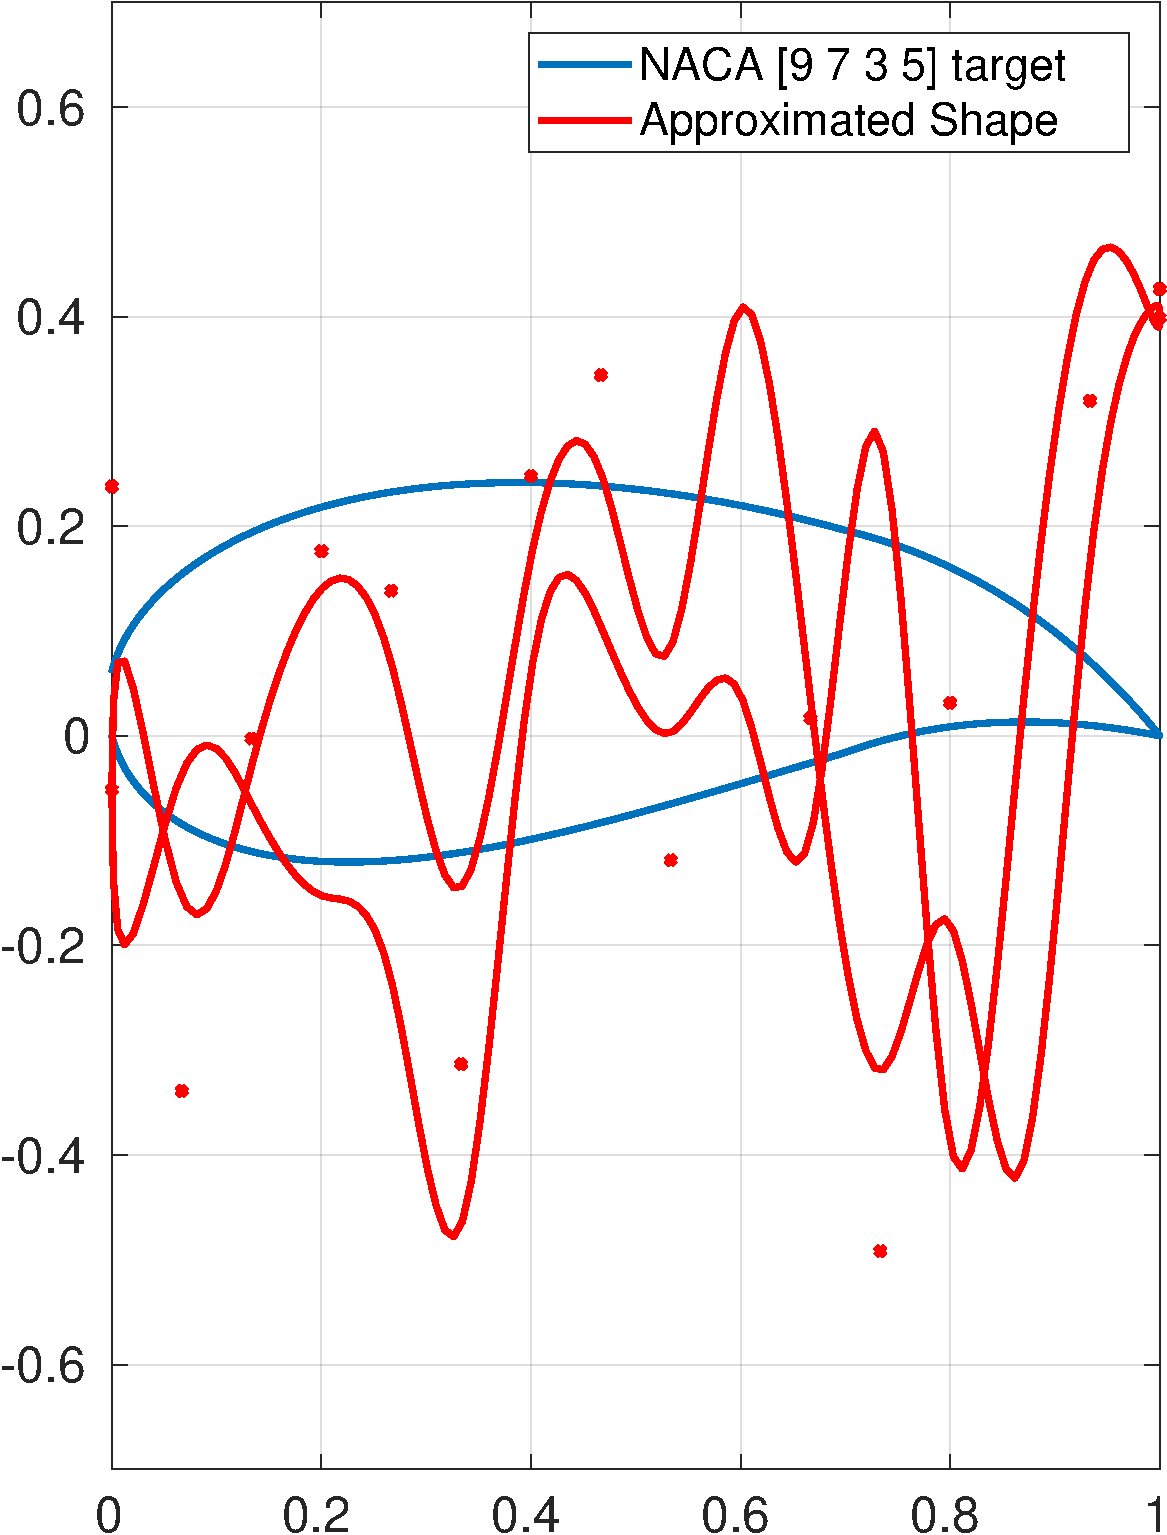
\includegraphics[width=.95\linewidth]{a3-shapematch-9735-init}
        \captionof{figure}{Initialized solution for the 9735 shape}
        \label{fig:initial}
    \end{minipage}%
    \begin{minipage}{.5\textwidth}
        \centering
        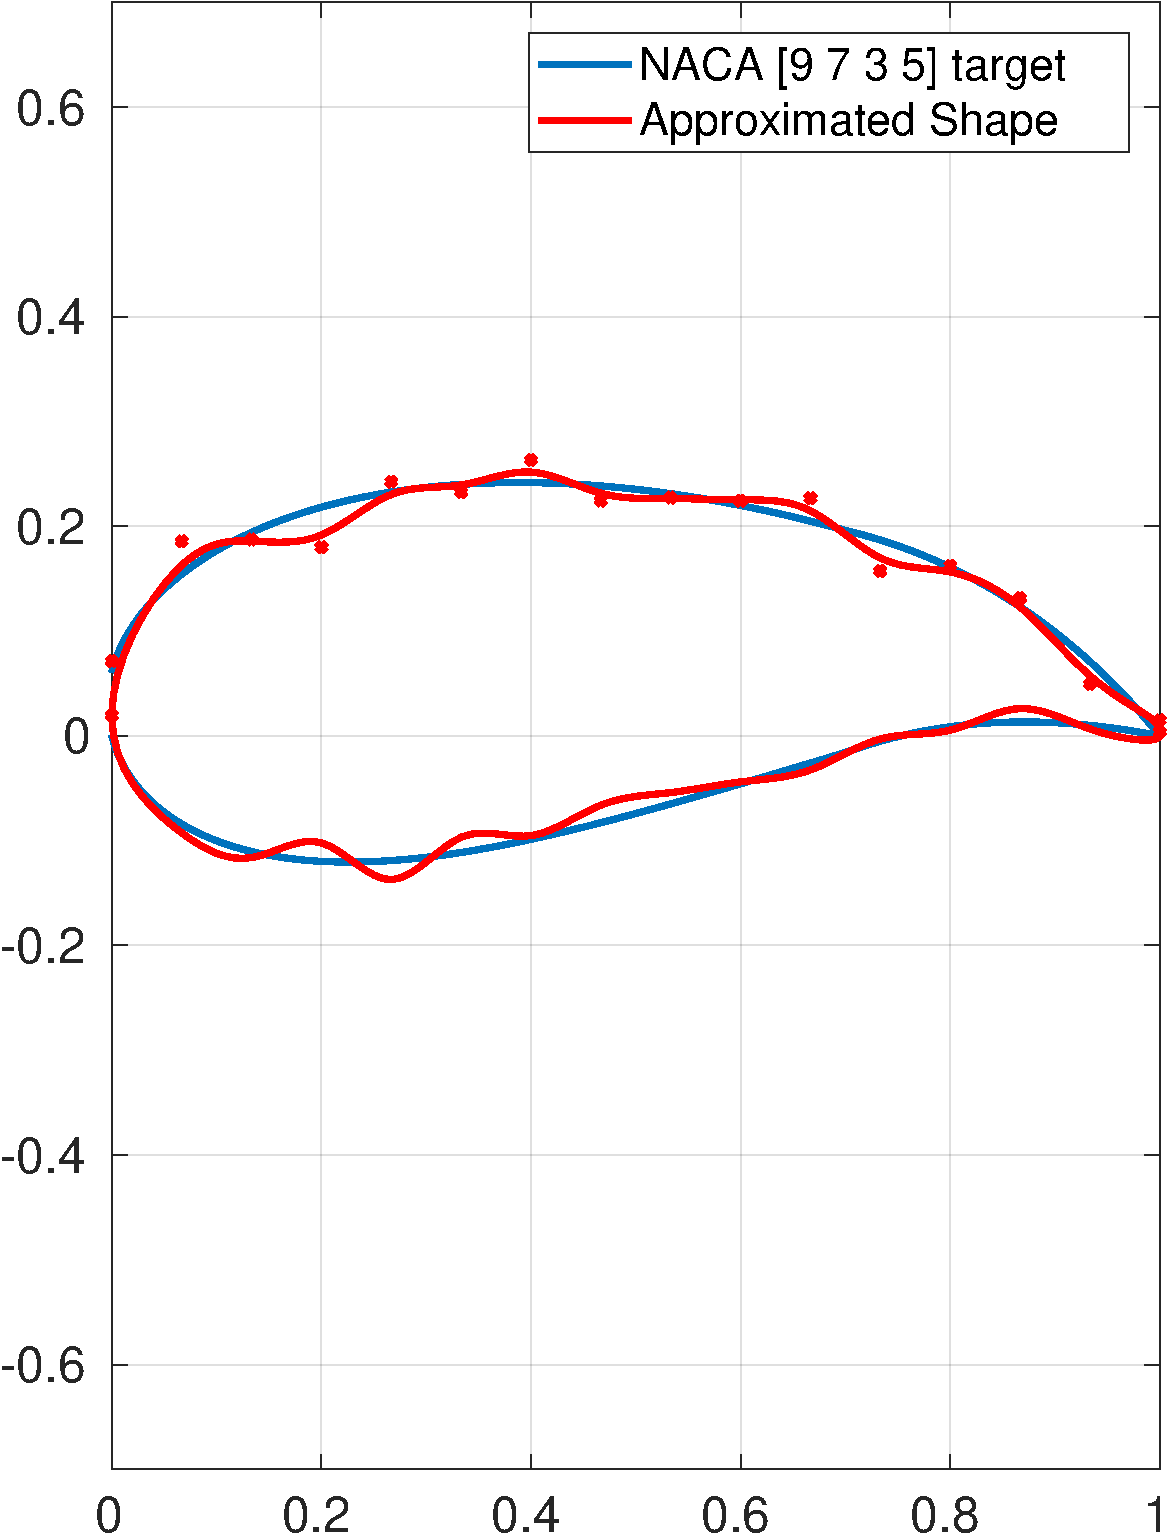
\includegraphics[width=.95\linewidth]{a3-shapematch-9735-final}
        \captionof{figure}{A final solution for the 9735 shape}
        \label{fig:solution}
    \end{minipage}
    \end{figure}
    The above solutions are the best after 3 runs of 1200 generations each.

    \section{Statistical Evaluation}

    The following box plot shows the fitness distribution of the best children after 30 runs of 1200 generations each for matching the 0012 NACA shape.

    \begin{figure}[h!]
        \centering
        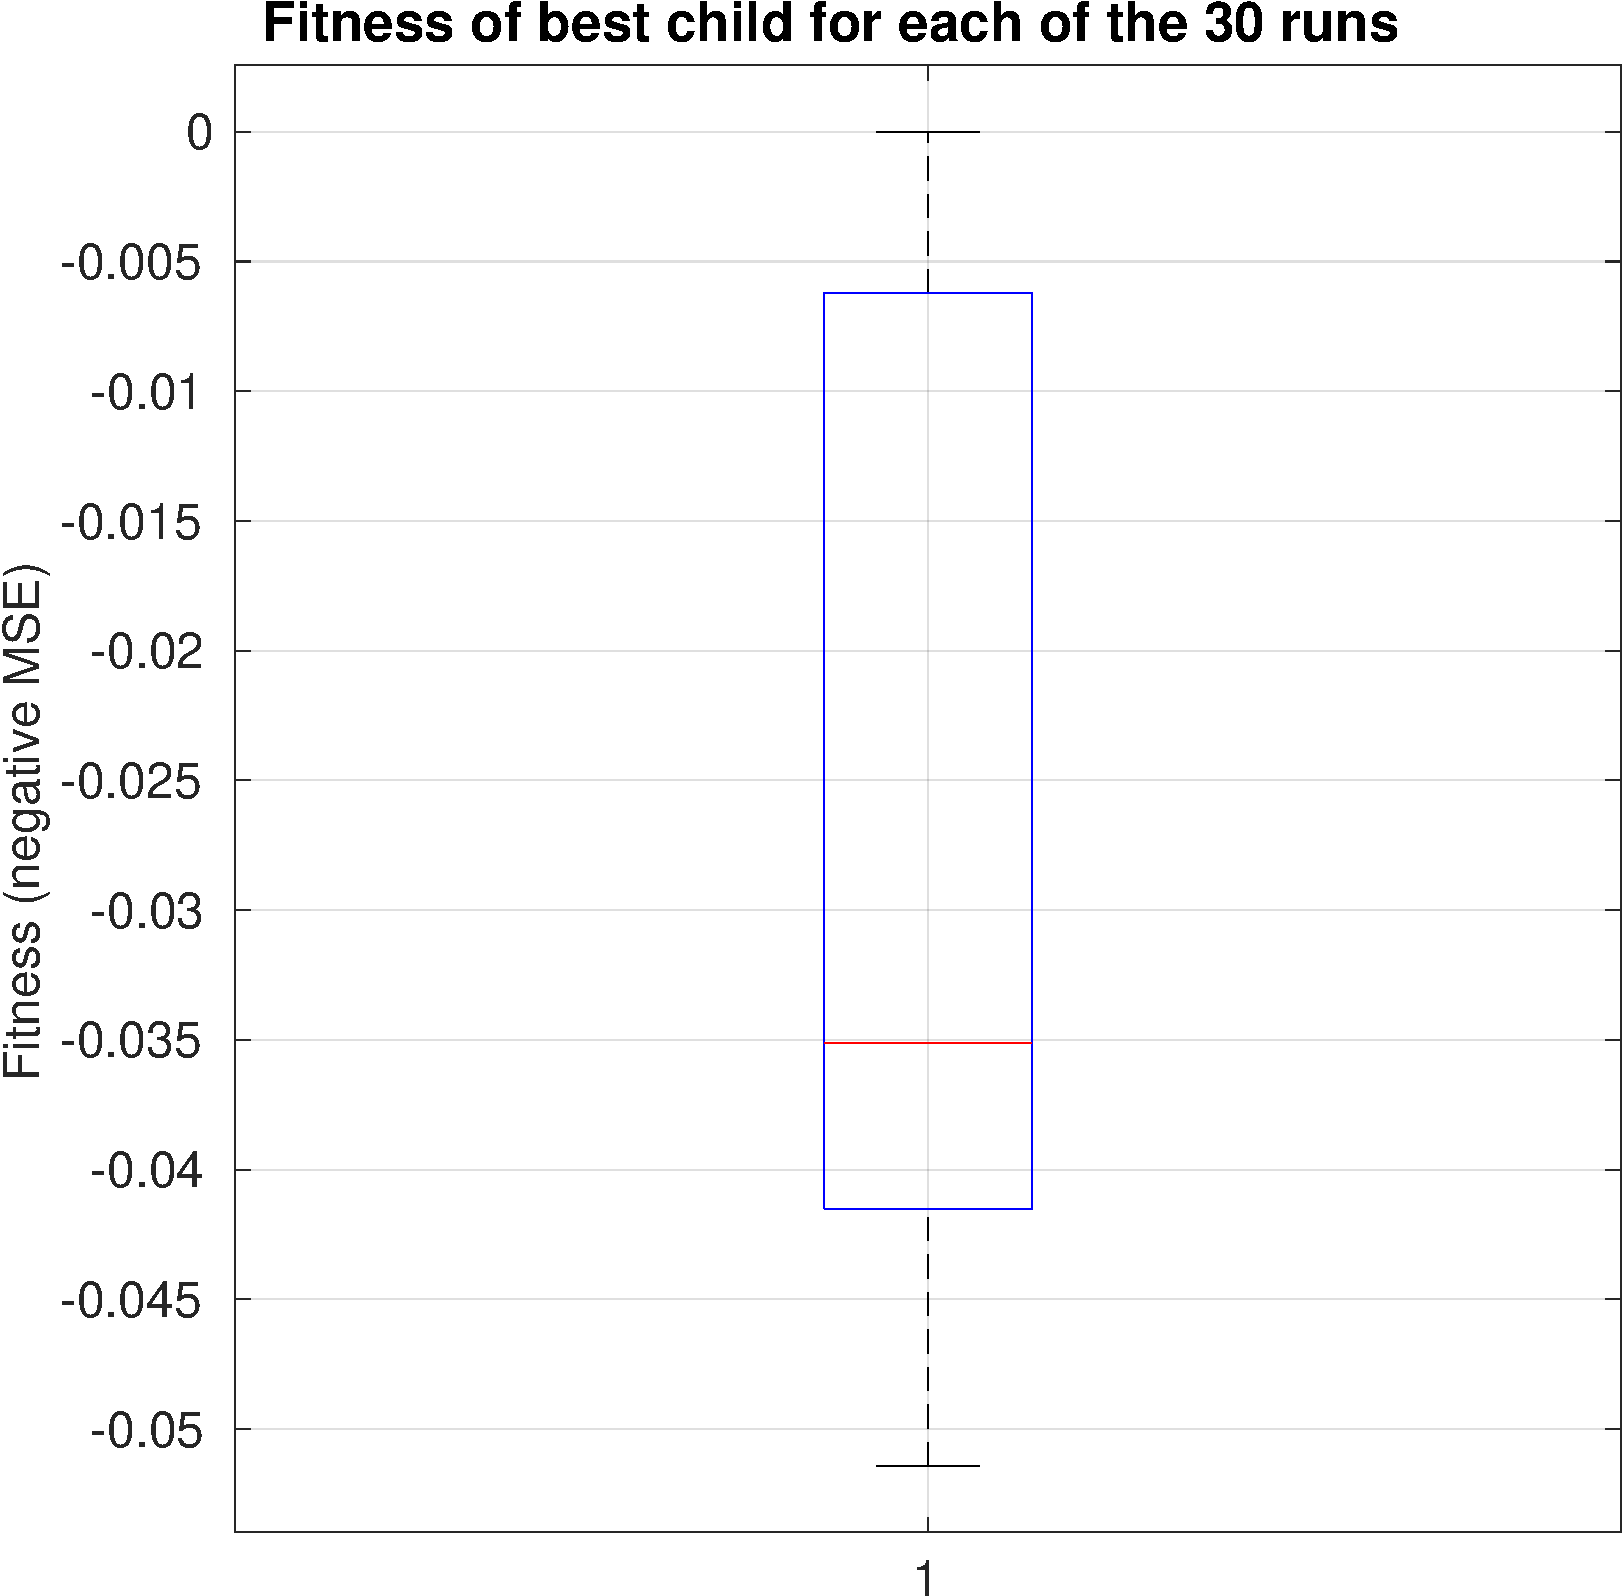
\includegraphics[width=.9\linewidth]{a3-shapematch-0012-bestChildrenFitnessBoxplot}
        \captionof{figure}{Box plot for the distribution of fitness of the best children over 30 runs}
        \label{fig:boxplot}
    \end{figure}
    \begin{figure}
        \centering
        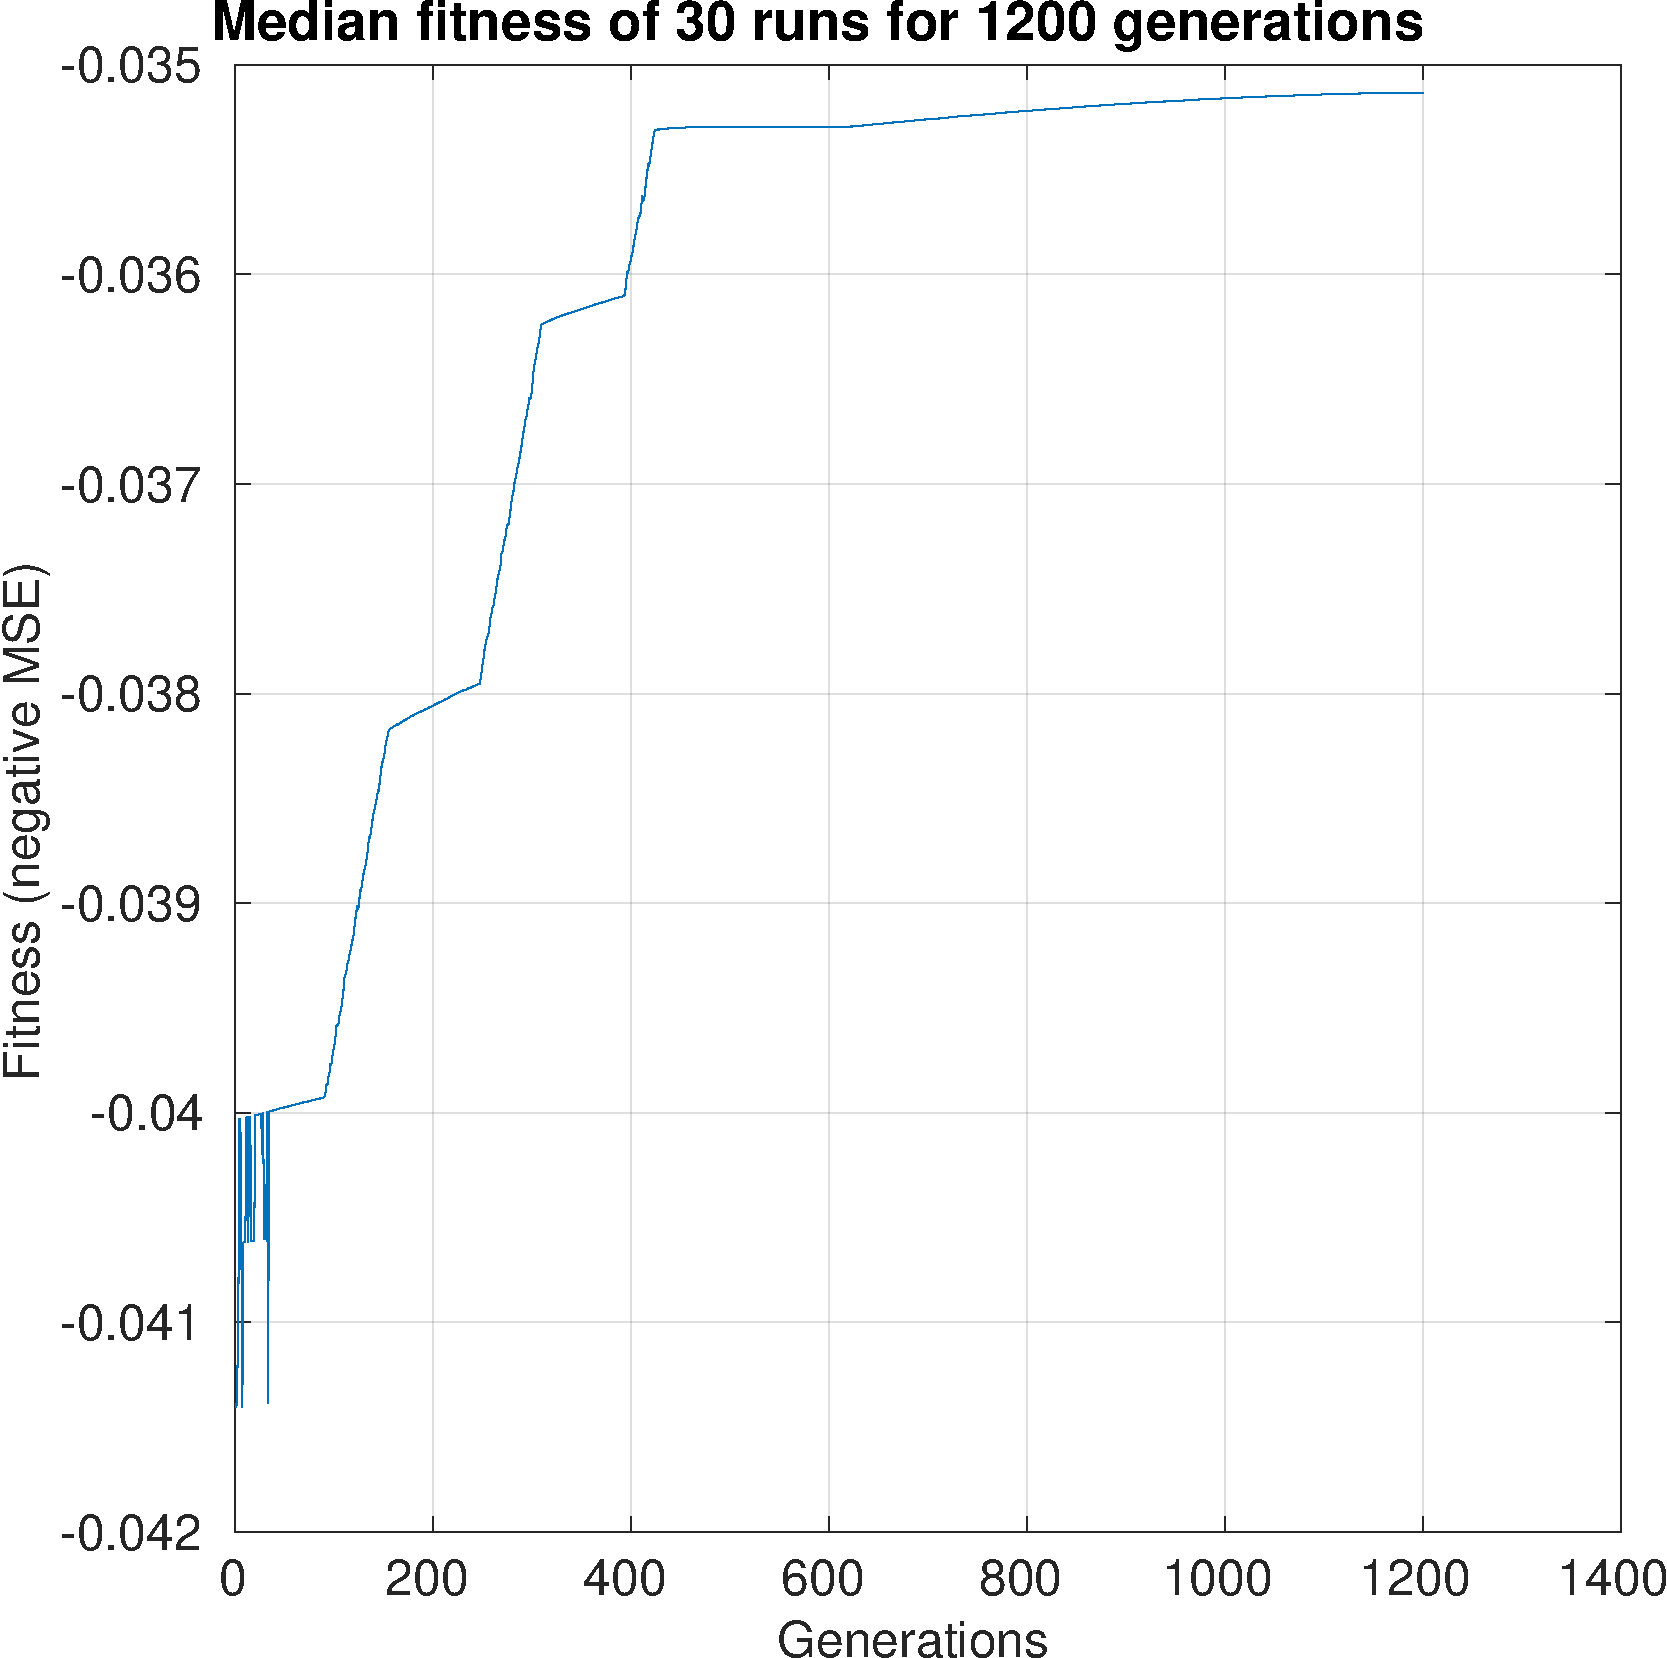
\includegraphics[width=.9\linewidth]{a3-shapematch-0012-fitness}
        \captionof{figure}{Median fitness progression over 30 runs of 1500 generations}
        \label{fig:median}
    \end{figure}

\end{document}
